%%%%%%%%%%%%%%%%%%%%%%%%%%%%%%%%%%%%%%%%%%%%%%%%%%%%%%%%%%%%%%%%%%
% Artigo segundo as normais mais atualizadas da ABNT
% Adaptado do projeto ABNTeX2 (que nao esta totalmente sincronizada com as normas da ABNT)
% Autor: Berg Dantas (bergdantas@msn.com)
%%%%%%%%%%%%%%%%%%%%%%%%%%%%%%%%%%%%%%%%%%%%%%%%%%%%%%%%%%%%%%%%%%
\documentclass[article,12pt,oneside,a4paper,english,brazil,sumario=tradicional]{abntex2}		
% Pacotes usados
\usepackage{times}%Usa a fonte Latin Modern
\usepackage[T1]{fontenc}%Selecao de codigos de fonte.
\usepackage[utf8]{inputenc}%Codificacao do documento
\usepackage{indentfirst}%Indenta o primeiro parágrafo de cada seção.
\usepackage{nomencl}%Lista de simbolos
\usepackage{color}%Controle das cores
\usepackage{graphicx}%Inclusão de gráficos
\usepackage{microtype}%Para melhorias de justificação
\usepackage{lipsum}%Para geração de dummy text
\usepackage[abnt-emphasize=bf,abnt-and-type=e,alf]{abntex2cite}%Citações ABNT
\usepackage{mathptmx}
\usepackage{enumitem}
%\usepackage[bottom=2cm,top=3cm,left=3cm,right=2cm]{geometry}

% Configuracoes do documento
\graphicspath{{./Figuras/}}%Images na pasta "Figuras"
\setsecheadstyle{\bfseries \normalsize \uppercase}
\setsubsecheadstyle{\normalsize \uppercase}
\setsubsubsecheadstyle{\bfseries \normalsize}
\setlrmarginsandblock{3cm}{2cm}{*}%Margens esquerda-direita
\setulmarginsandblock{3cm}{2cm}{*}%Margens cima-baixo
\checkandfixthelayout
\setlength{\parindent}{1.25cm}%paragrafo
\OnehalfSpacing%espacamento de 1,5
\setlength{\ABNTEXcitacaorecuo}{4cm}%recuo citacao direta +3

\begin{document}
\selectlanguage{brazil} % Seleciona o idioma do documento
\frenchspacing % Retira espaço extra obsoleto entre as frases.

    \begin{center}

    \begin{figure}[!ht]%[!htbp]
    \begin{center}  
    
\includegraphics[scale=0.8]{Figuras/LogoTitle4.png}
    \end{center}
    \end{figure}

	{\uppercase{\bfseries{ANÁLISE DA GESTÃO DE ESTOQUE  EM  UMA LOJA DE MATERIAL DE CONSTRUÇÃO DE MANAUS}}
	\vspace{14pt}}
	
	{
	Karen Silva; Jonas Gomes da Silva\\
	Universidade Federal do Amazonas - UFAM - Manaus/AM - Brasil\\
	karen.silva.eng@gmail.com e gomesjonas@hotmail.com
	\vspace{12pt}}

\end{center}


%\begin{flushright}
%AUTOR - Pode-se contar com infinitos autores   :)
%	Karen Silva\footnote{UFAM, karen.silva.eng@gmail.com}
%	\\
%	Jonas Gomes\footnote{UFAM, gomesjonas@hotmail.com}
%	\vspace{12pt}
%\end{flushright}

\begin{footnotesize}
\SingleSpacing
\noindent
\small{\textbf{Resumo:}}
\noindent
\small
%TEXTO DO RESUMO (em português}
Resumo resumo resumo resumo resumo resumo resumo resumo resumo resumo resumo resumo resumo resumo resumo resumo resumo resumo resumo resumo resumo resumo resumo resumo resumo resumo resumo resumo resumo resumo resumo resumo resumo resumo resumo resumo resumo resumo resumo resumo resumo resumo resumo resumo resumo resumo resumo resumo resumo resumo resumo resumo resumo resumo resumo resumo resumo resumo resumo resumo resumo resumo resumo resumo resumo resumo resumo resumo resumo resumo resumo resumo resumo resumo resumo.

\noindent
%PALAVRAS-CHAVE} 
\textbf{Palavras-chave}: Gestão de estoque, Problemas no estoque e Avaliação da gestão de estoque.
\end{footnotesize}

\textual
\pagestyle{simple}
\aliaspagestyle{chapter}{simple}

%=-=-=-=-=-=-=-=-=-=-=-=-=-=-=-=-=-=-=-=-=-=-=-=-=-=-=
\section{Introdução}
\label{chapter:secao1}
%=-=-=-=-=-=-=-=-=-=-=-=-=-=-=-=-=-=-=-=-=-=-=-=-=-=-=

\normalsize
Em tempos de grandes investimentos e crescimento econômico, a busca por diferenciais para garantir aumento das operações e/ou adquirir melhor qualidade de produtos e serviços, sempre foram fatores que instigavam a pesquisa e aplicação de recursos.

Nos dias atuais, com o país saindo de uma severa recessão econômica, essa busca tem aumentado. Os setores que mais buscam inovações são indústria e comercio. Com cada vez mais pessoas buscando seu próprio empreendimento, a competitividade tende a aumentar nos setores de comercio e serviços. Especificamente sobre materiais de construção, no Amazonas encontram-se cerca de $920$ lojas 
~\cite{AMANCO2014}.

O valor total das vendas de materiais de construção no comércio alcançou $R\$119,3$ bilhões em $2016$. Na comparação com o ano anterior houve queda nominal de $4,2$ ~\cite{ABRAMAT2017}.

No comercio as inovações afetam todos os setores dentro do estabelecimento, indo deste as técnicas de vendas, o pós venda e gestão de estoque. Segundo o Sindicato do Comércio Atacadista de Louças, Tintas e Ferragens de Manaus (Simacon), em janeiro de $2017$, havia na cidade de Manaus, 297 lojas de materiais de construção associadas ao sindicato ~\cite{SIMACON2017}.

Em uma loja de materiais de construção, o maior desafio é a gestão de estoque. Evitar que produtos atinjam seu prazo de validade, má conservação, FIFO não efetivo \textcolor{red}{.... (melhorar)}

Segundo, \citeonline{Pascoal2008}, para se manter um estoque organizado, são necessários vários requisitos, uns dos principais são: determinar o número de itens que deve ser estocados, a quantidade necessária para um período determinado e qual o momento certo que deve reabastecer o estoque. E toda a empresa deve ter um estoque mínimo ou também chamado de estoque de segurança, que determina a quantidade mínima estocada, que é destinada caso tenha algum atraso no momento da compra com o fornecedor, garantindo um funcionamento eficiente da empresa, sem riscos de falta ao consumidor.

Desse modo, para que uma empresa tenha um bom desenvolvimento é preciso que tenha uma boa gestão de estoques, controlando e armazenando adequadamente os materiais, para que não haja falhas e posteriormente a falta do produto. Diante disso, o objetivo principal desse trabalho foi analisar a gestão de estoque de uma empresa de materiais de construção localizada no bairro Aleixo na cidade de Manaus. Foi realizado uma pesquisa a partir de observações e um questionário semi-estruturado, para saber pelos próprios funcionários quais seriam os problemas de estoque na empresa em questão. Observaram-se vários problemas de gestão de estoques, como: esquecimentos de materiais pela falta de organização e o principal agravante desta empresa é que todo o processo de contagem de estoques e vendas é feita manualmente, possibilitando assim muitas falhas. 
Desse modo, o trabalho apresentado explicitará quais são os problemas de uma empresa que não tem uma gestão de estoque definida e quais seriam as sugestões possíveis para que se tenha um bom desenvolvimento dentro do estoque e como isso facilitaria a sua gestão.

%=-=-=-=-=-=-=-=-=-=-=-=-=-=-=-=-=-=-=-=-=-=-=-=-=-=-=
\section{Referencial Teórico - Definir Tópico}
\label{chapter:secao2}
%=-=-=-=-=-=-=-=-=-=-=-=-=-=-=-=-=-=-=-=-=-=-=-=-=-=-=

\subsection{Gestão de Estoque}
\label{subsection:gestaoEstoque}

\citeonline{Correa2004} nos dizem que, quando as empresas possuem um estoque grande ela pode atender com mais facilidade uma grande quantidade de clientes. No entanto, como saber qual produtor estocar? E a quantidade? 

Determinar essas variáveis (“o que?” e “quanto?” ter em estoque) é sempre uma adversidade enfrentada pelas empresas. Para determinar as demandas de produtos, as empresas, costumam fazer analise do histórico de vendas, afim de estimar quantidade e valor, de vendas futuras. 

Estoques em excesso geram grandes perdas de valor e gasto com armazenamento e mão de obra. Além de que, a mercadoria pode perder parte do seu valor ou perecer ocasionando grande prejuízo para empresa.

Outo fator encontrado em um grande volume de estoque é o espaço para o armazém. Quanto maior o estoque maior será o espaço utilizado pela empresa para guardar esse volume.

O objetivo da gestão de estoque é assegurar um nível adequado de estoque, que seja capaz de sustentar o nível de atividades da empresa ao menor custo. 
\citeonline{Matias2007} observa que os estoques servem para melhorar o atendimento as necessidades da empresa, em um espaço curto de tempo, e a um baixo preço. 

Segundo \citeonline{Correa2004}, várias empresas na década de 1980 tentaram manter estoques mínimos, gerando problemas de abastecimentos e paradas de produção e suspensão de serviços. Formulou-se, na época, a ideia que grande volume em estoque era um desperdício de espaço e dinheiro parado. Está ideia não está totalmente errada, está incompleta. O estoque deve ser aquele que foi estipulado pela empresa.

Trabalhar com estoque mínimo é vantajoso quando os fornecedores de matéria prima se encontram nas proximidades da empresa, e existe confiança nos prazos de entrega. Manter um estoque de segurança é uma maneira que as organizações não criarem custos adicionais. 

O método just in time é um modo de gestão de estoque, onde as empresas buscam diminuir o tempo de fabricação e o tamanho de seus estoques. De origem japonesa, este modelo foi implementado na administração da organização para ajudar na redução de custo para as empresas e seus fornecedores \cite{MAXIMIANO2005}.

Campos (2013) pontuam parâmetros para gerir estoques, que são:
\begin{enumerate}[label=\alph*)]
\item \textbf{Consumo Médio} – É a média aritmética do consumo previsto ou realizado num determinado período.
\item \textbf{Tempo de Reposição} – É o prazo dado desde a emissão de ordens de compra até o atendimento.
\item \textbf{Lote de Encomenda (ou Econômico)} – É a quantidade de material que se compra ou se fabrica de cada vez. Deve-se procurar um tamanho de lote que minimize o custo total anual.
\item \textbf{Estoque de Segurança} – Este é um item delicado que leva em conta a previsão de variação no consumo médio e, também, no tempo de reposição, para equilibrar a reserva de estoque de um lado e os custos de oportunidade de outro.
\item \textbf{Estoque Máximo} - É a quantidade máxima de material a ser mantida em estoque, é a soma do Lote de Encomenda com o Estoque de Segurança. 
\end{enumerate}


\subsubsection{Gestão Visual}
\label{subsubsection:gestaoVisual}

A gestão à vista é uma metodologia ligada à preocupação com a qualidade no trabalho. O programa 5s atua no sentido de permitir saltos de qualidade interna sejam dados por meio da prática da gestão à vista. 

A criação de uma cultura de bons hábitos deve fazer com que os colaboradores envolvidos absorvam as ideias e incorporem-nas como parte constante de sua rotina de trabalho, sempre atentando para os pontos do programa que necessitam de reavaliação e melhorias \cite{ABRANTES2001}. 

\citeonline{GREIF1989} diz que a gestão visual é um poderosa fonte de informação, ajuda a comunicar de forma rápida e eficazmente na empresa, mostrando indices e resultados dos esforços da organização. Comunicação visual é informação self-service – faz a mesma informação comumente disponível e compreensível a todos que a vêem, no exato momento em que a vêem \cite{GREIF1989}. 

A comunicação da informação deixa de estar restringida a um fluxo hierárquico, permitindo que o fluxo se crie por si só. Além disso o fluxo de informação da gestão visual é fundamental num processo de mudança de uma empresa, permitindo uma maior envolvimento de todos os colaboradores. 

Esta não está confinada apenas a quadros de indicadores, imagens instrutivas ou notas de precauções, mas a um conjunto de técnicas que integram a informação nos sistemas operativos, de forma a adicionar valor a cada tarefa produtiva. 

Em suma, a gestão visual aliada a um programa de implementação Lean permite a eliminação dos três tipos de perdas identificados por \citeonline{DREW2004}, uma vez que permite a interpretação rápida e fácil da informação, uma resposta rápida aos problemas e a comunicação entre as equipas de trabalho. Contribui, assim, para uma maior autonomia dos operadores e redução de erros, que resulta numa melhoria do ambiente de trabalho e na unificação da cultura empresarial.



%Na se\c c\~ao de desenvolvimento voc\^es usar\~ao muitas refer\^encias!!!

%\textbackslash nocite\{rotuloDaReferencia\}, faz com que uma cita\c c\~ao que n\~ao foi citada no texto apare\c ca nas Refer%\^encias Bibliogr\'aficas. \textbf{Exemplo de uso:} \textbackslash nocite\{tanebaum2010\} 

%De acordo\citeonline{tanebaum2010}, n\~ao importa o que ele disse. S\'o estou fazendo uma cita\c c\~ao indireta. 

%"($\cdots$) cita\c c\~ao direta com at\'e 3 linhas, cita\c c\~ao direta com at\'e 3 linhas, cita\c c\~ao direta com at\'e 3 linhas, cita\c c\~ao direta com at\'e 3 linhas, cita\c c\~ao direta com at\'e 3 linhas cita\c c\~ao direta com at\'e 3 linhas cita\c c\~ao direta com at\'e 3 linhas ($\cdots$)" \cite[p.~34]{tanebaum2010}.
 
%\vspace{24pt} %dois espacos de 12
%\begin{citacao}
%"Cita\c c\~ao direta com mais de 3 linhas, cita\c c\~ao direta com mais de 3 linhas, cita\c c\~ao direta com mais de 3 linhas, cita\c c\~ao direta com mais de 3 linhas, cita\c c\~ao direta com mais de 3 linhas, cita\c c\~ao direta com mais de 3 linhas, cita\c c\~ao direta com mais de 3 linhas, cita\c c\~ao direta com mais de 3 linhas, cita\c c\~ao direta com mais de 3 linhas, cita\c c\~ao direta com mais de 3 linhas, cita\c c\~ao direta com mais de 3 linhas, cita\c c\~ao direta com mais de 3 linhas, cita\c c\~ao direta com mais de 3 linhas, cita\c c\~ao direta com mais de 3 linhas, cita\c c\~ao direta com mais de 3 linhas. \cite[p.~34]{tanebaum2010}. 
%\end{citacao}
%\vspace{24pt} %dois espacos de 12

%Quando for preencher o arquivo "referencias.bib", no campo "author", se houverem dois ou mais autores, preenche os nomes normalmente separando-os por "and". Exemplo: \textit{Berg Dantas and Juliana Schivani}. Deve-se fazer isso sempre. Caso haja mais de 3 autores, o latex seleciona sozinho o primeiro e completa com o \textit{et al.} (significa "e outros" em latim). 

%\subsection{Materiais}
%Materiais materiais materiais materiais materiais materiais materiais materiais materiais materiais materiais materiais materiais.

%\subsection{M\'etodo}
%M\'etodo m\'etodo m\'etodo m\'etodo m\'etodo m\'etodo m\'etodo m\'etodo m\'etodo m\'etodo m\'etodo m\'etodo m\'etodo.

%\subsubsection{Testes}
%Testes testes testes testes testes testes testes testes testes testes testes testes testes testes testes testes testes.


%=-=-=-=-=-=-=-=-=-=-=-=-=-=-=-=-=-=-=-=-=-=-=-=-=-=-=
\section{Metodologia de coleta e análise de dados}
\label{chapter:METODOLOGIA}
%=-=-=-=-=-=-=-=-=-=-=-=-=-=-=-=-=-=-=-=-=-=-=-=-=-=-=

\subsection{Perfil da Empresa}
\label{subsection:perfil_empresa}

\subsection{Coleta de Dados}
\label{subsection:coleta_dados}


\subsection{Análise de Dados}
\label{subsection:analise_dados}






%\textcolor{red}{A pesquisa foi realizada entre dezembro de 2017 a abril de 2018 na loja de materiais de construção, IHS Materiais de Construções.}

%\textcolor{red}{A Empresa IHS Materiais de Construções, constitui-se em uma Empresa de Pequeno Porte situada na cidade de Manaus-AM, no bairro Aleixo, na qual se trabalha com uma gama de produtos essenciais a uma obra, desde materiais básicos (produtos mais pesados, tais como, areia, tijolos, cimentos, ferragens, madeiras, etc.) até produtos para acabamento (produtos mais leves, tais como pincéis, tintas, pias, conexões, entre outros).}

%\textcolor{red}{A loja possui 50 metros de frente por 30 metros de fundo, numa parte da cidade onde o comércio de materiais de construção é bastante intenso. Convém ressaltar que a empresa teve sua fundação no ano de 2000, porém em um tamanho físico menor se comparado ao disponível atualmente, visto que, por ser uma empresa familiar, veio crescendo fisicamente aos poucos, sem ter um planejamento inicial para a construção da mesma, fato que até hoje influencia na organização e disposição dos produtos no interior da loja, os quais, muitas vezes, não estão dispostos da melhor maneira. } 

%\textcolor{red}{Para o desenvolvimento desta pesquisa, o método utilizado foi o estudo de caso, caracterizado como uma investigação empírica de fenômenos contemporâneos no contexto real, em especial quando os limites entre fenômenos e o contexto não são evidentes. }

%\textcolor{red}{Para orientar a da coleta dos dados e aumentar a confiabilidade da pesquisa. \citeonline{YIN2010} sugere o protocolo de estudos de caso, no qual deve conter: visão geral do projeto do estudo de caso, questões do estudo de caso e leituras importantes sobre o tópico a ser investigado, conter as questões específicas para a coleta de dados, planilha para disposição de dados e fontes para responder a cada questão. }

%\textcolor{red}{A análise do estudo de caso, possibilitou a triangulação das fontes de várias evidências permitindo assim a realização de apontamentos positivos e oportunidade de melhoria do processo para a elaboração das conclusões e na e obtenção dos resultados.}


%=-=-=-=-=-=-=-=-=-=-=-=-=-=-=-=-=-=-=-=-=-=-=-=-=-=-=
\section{ Discusso dos resultados}
\label{chapter:resultados}
%=-=-=-=-=-=-=-=-=-=-=-=-=-=-=-=-=-=-=-=-=-=-=-=-=-=-=


%\textcolor{red}{ Diante do cenáro atual da loja convém a realização de pequenas, mas eficientes mudanças e adaptações na gestão visual da loja, com o objetivo de diminuir movimentações desnecessárias de produtos e pessoas, além de evitar a interrupção do fluxo de clientes no interior da loja. Tais mudanças irão influenciar diretamente na satisfação dos clientes com a otimização do tempo de entrega, além de reduzir os custos de embarque, desembarque e custos por atrasos. Na análise organizacional desta empresa verificou-se que os produtos além de não estarem bem dispostos, geralmente não estão agrupados por família, ou seja, encontram-se dispersos. }

%\textcolor{red}{Pôde-se identificar também que o depósito não possui nenhuma ferramenta específica de controle de estoques, mas sim um sistema de informação geral da organização, que deveria ser alimentado corretamente, mas que pela falta de atualização de forma precisa, ocorrem falhas no controle de estoque. Segundo o gestor isso ocorre porque a empresa ainda está passando por um processo de mudança em seus sistemas de informatização. }

%\textcolor{red}{O gestor complementou ainda que já teve prejuízos por não conseguir controlar seus estoques corretamente, e que chegou a perder vendas e até clientes.}


%\subsection{Gestão de Estoque}
%\label{subchapter:GestãoEstoque}

%A primeira ação a ser feita na gestão de estoque foi a escolha de um sistema de controle do estoque.  
%A gestão da empresa optou por um sistema próprio, IHL, que tem funções de cadastro, 
%controle de entrada e saída, conseguindo gerar relatórios de vendas diários, semanal, mensal e anual 
%~\ref{fig:telaBuscaProduto}~\ref{fig:telaConsultaPreco}~\ref{fig:telaCompras}. 


%\begin{figure}[htb]
%\centering
%
\includegraphics[width=0.3\columnwidth]{Figuras/telaBuscaProduto.jpg}
%\label{fig:telaBuscaProduto}
%\caption{Tela IHS, Busca de produto }
%\end{figure}

%\begin{figure}[htb]
%\centering
%
\includegraphics[width=0.3\columnwidth]{Figuras/telaConsultaPreco.png}
%\label{fig:telaConsultaPreco}
%\caption{Tela IHS, Consulta Preço}
%\end{figure}

%\begin{figure}[htb]
%\centering
%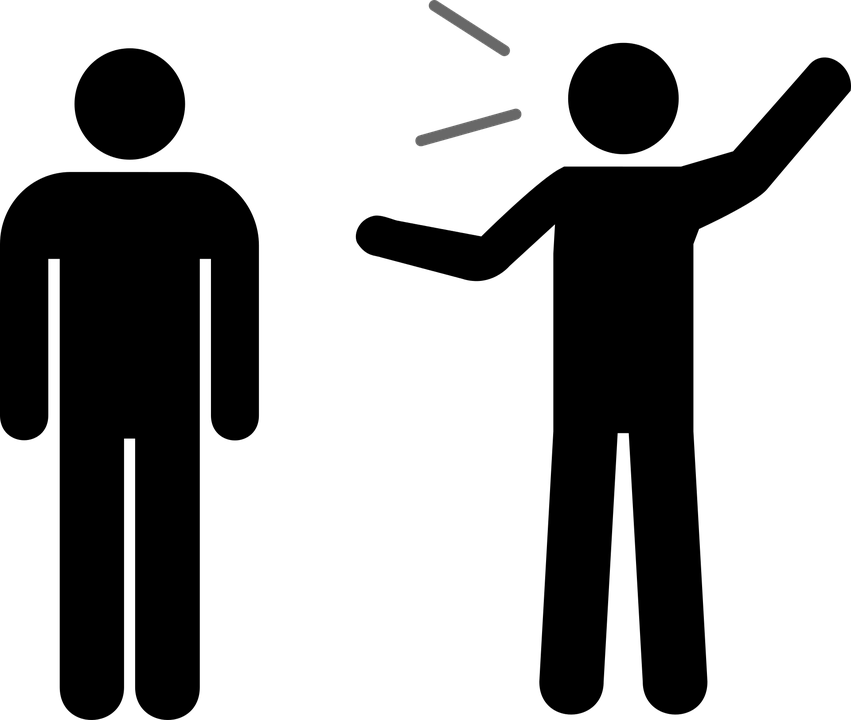
\includegraphics[width=0.3\columnwidth]{Figuras/telaCompras.jpg}
%\label{fig:telaCompras}
%\caption{Tela IHS, Compras }
%\end{figure}


%Com os dados em estoque, foi possivel observar as perdas por validade, por quebras e por outros, neste quesito coloca-se, roubo, furto e não conferencia de mercadorias (saída e entrada). Com os relatorios gerados podemos agora efetuar inventarios cicliclos.

%No diagnostico incial, a cada 25 itens verificados, tinha-se variação, nas quantidades em estoque, em 13,5 itens de média. Ocasionando um perda de receita de R\$18,500,00 (em média). Essas perdas, não contabilizadas anteriomente, deixaram de agregar $15\%$ no valor das vendas da empresa. 
%Os pedidos entregues errados aconteciam em $45\%$ das vezes, com o controle de estoque.

%A partir do momento em começamos a fazer o controle de estoque, as perdas no estoque tiveram uma queda, melhorando o FIFO e diminuindo a margem de erros de estoque. Diminui-se para quase zero a existencia de produtos vencidos em estoque. 

%A freqüência com que esses dados estiveram em observação foi quinzenalmente pelo tempo de três meses. 

%Nesta etapa a parte foi colocada em prática o controle de estoque, mas, o projeto que foi desenvolvido para a empresa é um projeto bem amplo que envolve todos os deptos como: Controle de estoques, Pagamentos, Recebimentos, e dentro de todos esses programas contém relatórios detalhados de todas as informações necessárias para se tomar decisões, quer seja para comprar algum item, saber se tem alguma mercadoria que sua venda é muito baixa, entre outras informações.


%\subsection{5S}
%\label{subchapter:5S}

%Com a coleta de dados conseguimos identificas os problemas das empresas e buscou-se a implantação das melhorias.

%O programa 5S foi escolhido para iniciar as melhorias de gestão visual da loja, atacando o layout da loja e reformulando a exibição de produtos. O 5S quando bem implantado, permite que a empresa consiga atingir liberação de espaço físico, melhoria do ambiente de trabalho, maior visualização dos materiais e organização.

%O primeiro senso que utilizamos foi o de limpeza, seguido a de utilização e arrumação. Com a a limpeza do ambiente, achamos avarias em produtos, produtos caidos, e contaminação por poeiras, substancias oleosas. Primeiro passo foi a eliminação das contaminações e limpenza dos produtos do mostruario.

%A seguir fomos definir a utilização dos produtos. No mostruario é adequado manter apenas um item de cada produto para que os consumidores possam verificar o mix de produto que a loja dispoem. O senso de ordenação foi o passo mais desafiador dado que o layout apresenta restrições que demandam estudos para suas soluções. As gondolas na entrada da loja, forma coloados os itens de menor valor e maior saída, conexões hidraulicas ( enroscadas e soldaveis). Indetificados com etiquetas para identificação dos mesmos. 

%Dando continuidade a arrumação da loja, seguimos por distribuir e alocar os materiais em quatro corredores de acordo com familias  a que o item pertence. Um corredor para ferramentas, outro para eletrica, o seguinte para  hidraulica e o quarto corredo para tintas. Com essa organização da loja, o cliente conseguiam percorrer a loja e identificar a possivel localização dos itens que procura. Os sensos de higiene e auto disciplina requerem uma aior concentração de esforços. 

%s colaboradores são bem particpativos e entendem que a melhoria da empresa, representa melhoria no ambiente de trabalha bem como possivel expansão e promoções internas. Os colaboradores receberam uniformes (camisa e bota) e epi’s (protetor auricular, oculos e cinta ortopedica) para uso no ambiente de trabalho.Além disso foram distribuidos kits para os vendedores, que inclui, lápis, marca texto, caneta esferografica, bloco de notas e agenda.

%Após aplicação do programa o monitoramente se manteve para assegurar que as ações implantadas sejam usadas e mantidas. Com o layout da loja, observou-se um crescimento no numero de vendas  de 14% durante a semana e 23% aos fds e feriados. Ainda que a receita proveniente de vendas tenha subido apenas 8%.


\renewcommand{\bibsection}{\section*{REFER\^ENCIAS BIBLIOGR\'AFICAS}}
\bibliographystyle{abntex2-alf}
\bibliography{Referencias}
\end{document}
